% !TeX root = ../libro.tex
% !TeX encoding = utf8
%
%*******************************************************
% Introducción
%*******************************************************
% \manualmark
% \markboth{\textsc{Introducción}}{\textsc{Introducción}} 
\addchap{Introducción}

\paragraph{\spacedlowsmallcaps{Contexto}}
\phantom{}

\begin{quote}
    "\textit{El problema principal de la comunicación es reproducir en un punto, ya sea de forma exacta o aproximada, un mensaje en otro punto.}"
\end{quote}

Con estas palabras comenzada Claude Shannon en 1948 el artículo ``A mathematical theory of comunication'' \cite{Shanon}, un trabajo que supuso el inicio de dos disciplinas imprescindibles en la actualidad: la teoría de códigos y la teoría de la información. En este artículo Shannon demostró que, mediante una \emph{codificación apropiada de la información}, los errores inducidos por un canal o medio ruidoso pueden \emph{reducirse a cualquier nivel deseado} sin empeorar la tasa de transmisión. El trabajo de Shannon proporcionó un marco teórico sobre la transmisión eficiente y fiable de la información.

Aunque el primer trabajo publicado de teoría de códigos fue el de Shannon, el verdadero padre de esta teoría es Richard W. Hamming, a quien Shannon nombró en su artículo. En 1950\footnote{Aunque el artículo de Hamming fue publicado en 1950, realmente es un trabajo anterior al de Shannon.}, motivado por la necesidad de corregir los errores producidos durante las operaciones con grandes números, Hamming publicó el artículo ``Error detecting and error correcting codes’’ \cite{Hamming}. Hamming introdujo un tipo de códigos llamados \emph{códigos de Hamming}, los cuales permiten detectar hasta errores de dos bits y corregir errores de un bit.

La teoría de códigos se encarga del diseño de códigos para la transmisión y el almacenamiento de los datos. Su principal objetivo es garantizar que la información pueda ser transmitida o almacenada de manera eficiente y con la menor cantidad posible de errores, aun cuando esta se envía a través de canales con ruido.

Supongamos que deseamos transmitir un \emph{mensaje}. En este caso, habrá un \emph{emisor} y un \emph{receptor} que se comunican, generalmente, de manera unidireccional. 
El mensaje consiste en una secuencia finita de símbolos de un alfabeto específico y se envía a través de un \emph{canal de comunicación}. Durante la transmisión, la información puede distorsionarse debido a interferencias o ruido presentes en el canal. Para mitigar este problema, es importante representar el mensaje en un formato adecuado para el canal, a la representación de este mensaje se le conoce como \emph{palabra código} y a este proceso de transformación de un mensaje en su palabra código correspondiente se le conoce como \emph{codificación}. Este proceso implica proteger el mensaje original mediante técnicas como la adición de redundancia, la repetición del mensaje o la incorporación de bits de paridad.
Una vez se ha codificado el mensaje, se envía a través de un \emph{canal}, donde puede sufrir alteraciones debido a la presencia de una \emph{fuente de ruido}. Al llegar el mensaje al \emph{receptor}, este recibe una versión posiblemente alterada de la palabra código original. Es entonces cuando se da el proceso conocido como \emph{decodificación}, que consiste en detectar y corregir los errores y transformar la palabra código corregida en el formato original.

Todo este proceso de transmisión está recogido en la Figura \ref{fig:comunicacion}.

\begin{figure}[H]
    \centering
    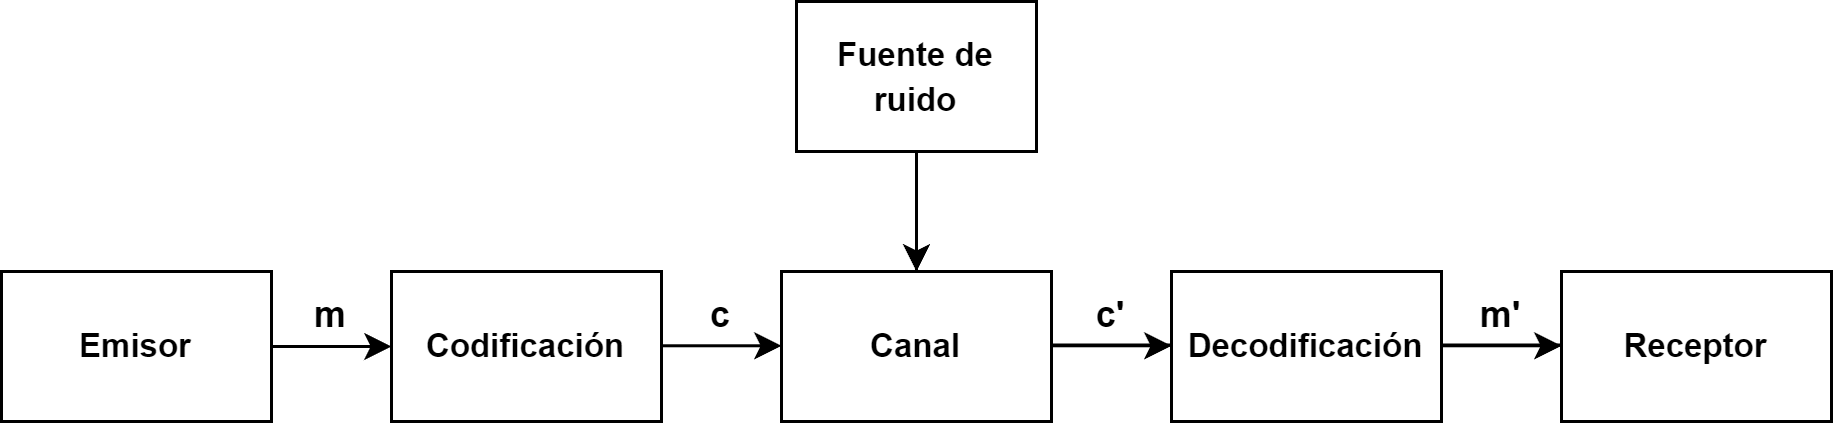
\includegraphics[width=1\textwidth]{img/comunicacion.png}
    \caption{Esquema del modelo de comunicación \cite{Podesta2006}.}
    \label{fig:comunicacion}
\end{figure}

En general, el mensaje enviado  y el mensaje recibido serán distintos. De esta forma, la teoría de códigos se encarga principalmente de los pasos de codificación y decodificación del diagrama anterior.

Algunas de las aplicaciones de la teoría de códigos son:

\begin{itemize}
    \item \emph{Comunicaciones digitales}: Se emplea en la telefonía móvil y redes de datos para asegurar la calidad y fiabilidad de las transmisiones.
    \item \emph{Almacenamiento de datos}: También es esencial el uso de códigos para garantizar la integridad de la información en discos duros, SSDs y medios ópticos como CDs y DVDs.
    \item \emph{Transmisiones por satélite}: Son imprescindibles también en todo tipo de transmisiones por satélite (televisión, GPS...), ya que protege de posibles interferencias atmosféricas.
    \item \emph{Criptografía}: Otro de sus usos más populares (y con el que a veces se confunde), es la criptografía. Por ejemplo, se utilizan en sistemas de cifrado asimétrico, como puede ser el criptosistema McEliece, que usa códigos de Goopa.
\end{itemize}


\paragraph{\spacedlowsmallcaps{Enfoque}}
\phantom{}

El objetivo principal de este trabajo es estudiar los códigos convolucionales cíclicos sesgados (SCCC) e implementar el algoritmo de Sugiyama para la decodificación de estos códigos. En consecuencia, el trabajo se enfocará en introducir las herramientas necesarias para poder abordar este objetivo. En cuanto a los fundamentos matemáticos necesarios, estudiaremos los anillos, los cuerpos finitos, los módulos y los anillos de polinomios sesgados. Para la teoría de códigos, veremos nociones básicas de los códigos de bloque, centrándonos en los códigos lineales y cíclicos. También hablaremos de códigos convolucionales, otra clase de códigos distinta a los de bloque, los cuales serán esenciales para la definición del objeto principal de este trabajo, los códigos convolucionales cíclicos sesgados.


\paragraph{\spacedlowsmallcaps{Estructura del trabajo}}
\phantom{}


Este trabajo consta de cinco capítulos y dos apéndices. En el primer capítulo, introduciremos los fundamentos matemáticos necesarios para desarrollar la teoría de códigos que se pretende abordar en este trabajo. En el segundo capítulo estudiaremos algunos de los fundamentos de los códigos de bloque, enfocándonos principalmente en los códigos lineales y cíclicos, presentando también el algoritmo de Sugiyama para la decodificación de códigos BCH, una subclase de los códigos cíclicos. En el tercer capítulo profundizaremos en los códigos convolucionales, explorando sus bases matemáticas y algunas de sus propiedades fundamentales. En el cuarto capítulo, veremos en primer lugar los polinomios de Ore, una estructura matemática que constituye la base de los códigos convolucionales cíclicos sesgados, que se introducen a continuación. Finalmente, en el quinto capítulo describimos el algoritmo de Sugiyama para la decodificación de códigos convolucionales sesgados Reed-Solomon.

En el primer apéndice, se detallará el código implementado en el trabajo, así como la estructura de este y los test realizados para probar su funcionamiento. En el segundo apéndice, se expondrá la planificación temporal del proyecto y una estimación de los costes del mismo.

\paragraph{\spacedlowsmallcaps{Objetivos principales del trabajo}}
\phantom{}

En cuanto al ámbito de las \emph{Matemáticas}, los objetivos de este trabajo son:

\begin{itemize}
    \item Estudiar las nociones básicas de la teoría de códigos lineales.
    \item Explorar los códigos convolucionales y su estructura algebraica, así como algunas de sus propiedades fundamentales.
    \item Investigar la noción de ciclicidad para los códigos convolucionales mediante los polinomios de Ore.
    \item Estudiar los códigos convolucionales sesgados Reed-Solomon.
    \item Exponer el algoritmo de Sugiyama para códigos convolucionales sesgados Reed-Solomon.
\end{itemize}

En cuanto a la \emph{Ingeniería Informática}, observemos que los objetivos anteriores se enmarcan en el campo de la Computación teórica. Además, otros objetivos más específicos son:

\begin{itemize}
    \item Implementar el algoritmo de Sugiyama para la decodificación de códigos BCH.
    \item Implementar un sistema de construcción de códigos convolucionales sesgados Reed-Solomon.
    \item Implementar un sistema de codificación de códigos convolucionales sesgados Reed-Solomon.
    \item Implementar el algoritmo de Sugiyama para la decodificación de códigos convolucionales sesgados Reed-Solomon.
\end{itemize}

\paragraph{\spacedlowsmallcaps{Principales fuentes consultadas}}
\phantom{}

Entre todas las fuentes bibliográficas consultadas, sobresalen las siguientes:

Para el estudio de las herramientas matemáticas del primer capítulo, \cite{knapp2006basic} y \cite{Huffman_Pless_2010} han resultado de utilidad.

En el segundo capítulo, \cite{Huffman_Pless_2010} y \cite{betten2006error} han sido fundamentales para el desarrollo de la teoría de códigos de bloque.

Para el capítulo tres, dedicado a los códigos convolucionales, las fuentes principales han sido \cite{Huffman_Pless_2010}, \cite{Forney1970}, \cite{Johannesson2015}, \cite{cccheide} y \cite{jl2020}.

En el capítulo cuatro, centrado en los códigos convolucionales cíclicos sesgados (SCCC), se han utilizado como referencias principales \cite{gluesingluerssen2019skewpolynomial} y \cite{jacobson1996} para los anillos de polinomios sesgados, además de \cite{cccheide}, \cite{SCCC} y \cite{gomez2017sugiyama} para los códigos convolucionales cíclicos sesgados.

Finalmente, el capítulo cinco, que aborda el algoritmo de decodificación Sugiyama para los códigos convolucionales sesgados Reed-Solomon, se basa en los resultados descritos en \cite{gomez2017sugiyama}. 

Para el desarrollo de la implementación y pruebas, ha sido relevante la documentación de SageMath \cite{SageMath2022} y Pytest \cite{pytest7.4.0}.






\endinput

